\newcommand{\sinPhase}[2] {
    \addplot[smooth, domain=0:360,line width=1.5pt, #2]{sin(x - (#1))};
}

\newcommand{\phase}[2] {
    \addplot[->, >=latex, line width=2.5pt, #2] coordinates { (0,0) (#1,1.5) };
}

\begin{center}
\begin{tabular}{rl}
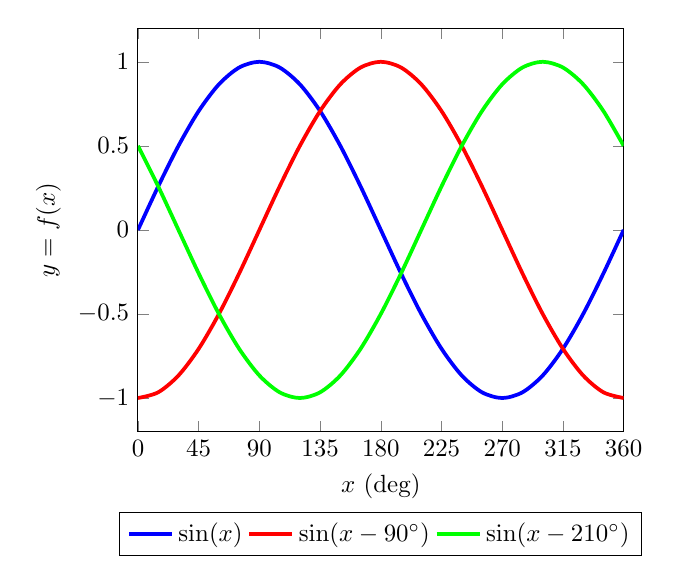
\begin{tikzpicture}[baseline,scale=0.9]
\begin{axis}[
    domain=0.0:360,
    xlabel={$x$ (deg)},
    ylabel={$y = f(x)$},
    xtick distance = 45,
    ytick distance = 0.5,
    enlarge x limits=false,
    legend style={at={(0.5, -0.2)}, anchor=north, legend columns=3},
]
    \sinPhase{0}{blue}
    \sinPhase{90}{red}
    \sinPhase{210}{green}
    \legend{$\sin(x)$, $\sin(x - 90^\circ)$, $\sin(x - 210^\circ)$}
\end{axis}
\end{tikzpicture}
&
\begin{tikzpicture}[baseline,scale=0.7]
\begin{polaraxis} [
    xlabel={Fázis (deg)},
    ytick = \empty,
]
    \phase{0}{blue}
    \phase{90}{red}
    \phase{210}{green}
\end{polaraxis}
\end{tikzpicture}
\end{tabular}
\end{center}
